\hypertarget{ux7406ux89e3-plonkux56dbux7b97ux672fux7ea6ux675fux4e0eux62f7ux8d1dux7ea6ux675f}{%
\chapter{算术约束与拷贝约束}\label{ux7406ux89e3-plonkux56dbux7b97ux672fux7ea6ux675fux4e0eux62f7ux8d1dux7ea6ux675f}}

\hypertarget{ux56deux987eux7f6eux6362ux8bc1ux660e}{%
\section{回顾置换证明}\label{ux56deux987eux7f6eux6362ux8bc1ux660e}}

上一节,我们讨论了如何让 Prover 证明两个长度为 \(N\) 的向量 \(\vec{a}\)
与 \(\vec{b}\) 满足一个实现约定(公开)的置换关系 \(\sigma(\cdot)\),即

\[
a_i = b_{\sigma(i)}
\]

基本思路是向 Verifier 要一个随机数
\(\beta\),把两个「原始向量」和他们的「位置向量」进行合体,产生出两个新的向量,记为
\(\vec{a}'\) 与 \(\vec{b}'\)

\[
a'_i = a_i + \beta \cdot i, \qquad b_i'=b_i+\beta\cdot \sigma(i)
\]

第二步是再向 Verifier 要一个随机数 \(\gamma\),通过连乘的方法来编码
\(\vec{a}'\) 和 \(\vec{b}'\) 的 Multiset,记为 \(A\) 和 \(B\):

\[
A = \prod(a'_i + \gamma),\qquad B = \prod(b'_i + \gamma)
\]

第三步是让 Prover 证明 \(A/B=1\),即

\[
\prod_i\frac{(a'_i + \gamma)}{(b_i'+\gamma)} = 1
\]

证明这个连乘,需要引入一个辅助向量
\(\vec{z}\),记录每次乘法运算的中间结果:

\[
z_0=1, \qquad z_{i+1}=z_i\cdot \frac{(a'_i+\gamma)}{(b'_i+\gamma)}
\]

由于 \(z_N=\prod\frac{a'_i+\gamma}{b'_i+\gamma}=1\),而且
\(\omega^N=1\),因此我们可以用 \(z(X)\) 来编码
\(\vec{z}\),从而把置换证明转换成关于 \(z(X), a(X)\) 的关系证明。

最后 Verifier 发送挑战数 \(\zeta\),得到
\(z(\zeta), z(\omega\cdot\zeta), a(\zeta), b(\zeta)\)
然后检查它们之间的关系。

\hypertarget{ux5411ux91cfux7684ux62f7ux8d1dux7ea6ux675f}{%
\section{向量的拷贝约束}\label{ux5411ux91cfux7684ux62f7ux8d1dux7ea6ux675f}}

所谓拷贝约束 Copy
Constraints,是说在一个向量中,我们希望能证明多个不同位置上的向量元素相等。我们先从一个简单例子开始:

\[
\vec{a}=(a_0, a_1, a_2, a_3)
\]

假设为了让 Prover 证明 \(a_0=a_2\),我们可以把 \(a_0\) 与 \(a_2\)
对调位置,这样形成一个「置换关系」,如果我们用 \((0,1,2,3)\)
记录被置换向量的元素位置,那么我们把置换后的位置向量记为 \(\sigma\) ,而
\(\vec{a}_\sigma\) 为表示按照 \(\sigma\) 置换后的向量

\[
\sigma=(2,1,0,3), \quad \vec{a}_\sigma=(a_2,a_1,a_0, a_3)
\]

显然,只要 Prover 可以证明置换前后的两个向量相等,
\(\vec{a}=\vec{a}_\sigma\),那么我们就可以得出结论: \(a_0=a_2\)。

这个方法可以推广到证明一个向量中有多个元素相等。比如要证明 \(\vec{a}\)
中的前三个元素都相等,我们只需要构造一个置换,即针对这三个元素的循环右移:

\[
\sigma=(2,0,1,3),\quad \vec{a}_\sigma=(a_2,a_0,a_1,a_3)
\]

那么根据 \(\vec{a}=\vec{a}_\sigma\) 容易得出 \(a_0=a_1=a_2\)。

\hypertarget{ux591aux4e2aux5411ux91cfux95f4ux7684ux62f7ux8d1dux7ea6ux675f}{%
\section{多个向量间的拷贝约束}\label{ux591aux4e2aux5411ux91cfux95f4ux7684ux62f7ux8d1dux7ea6ux675f}}

对于 Plonk 协议,拷贝约束需要横跨 \(W\) 表格的所有列,而协议要求 Prover
要针对每一列向量进行多项式编码。我们需要对置换证明进行扩展,从而支持横跨多个向量的元素等价。

%\includegraphics{img/img2020230414202348.png}

回忆比如针对上面电路的 \(W\) 表格:

\[
\begin{array}{c|c|c|c|}
i & w_a & w_b & w_c  \\
\hline
0 & 0 & 0 & {\color{green}out} \\
1 & {\color{red}x_6} & {\color{blue}x_5} & {\color{green}out} \\
2 & x_1 & x_2 & {\color{red}x_6} \\
3 & x_3 & x_4 & {\color{blue}x_5} \\
\end{array}
\]

看上面的表格,我们要求 \(w_{a,1}=w_{c,2}\), \(w_{b,1}=w_{c,3}\) 且
\(w_{c,0}=w_{c,1}\)。

支持跨向量置换的直接方案是引入多个对应的置换向量,比如上表的三列向量用三个置换向量统一进行位置编码:

\[
\begin{array}{c|c|c|c|}
i & id_{a,i} & id_{b,i} & id_{c,i}  \\
\hline
0 & 0 & 4 & {\color{green}8} \\
1 & {\color{red}1} & {\color{blue}5} & {\color{green}9} \\
2 & 2 & 6 & {\color{red}10} \\
3 & 3 & 7 & {\color{blue}11} \\
\end{array}
\]

置换后的向量为 \(\sigma_a, \sigma_b, \sigma_c\):

\[
\begin{array}{c|c|c|c|}
i & \sigma_{a,i} & \sigma_{b,i} & \sigma_{c,i}  \\
\hline
0 & 0 & 4 & {\color{green}9} \\
1 & {\color{red}10} & {\color{blue}11} & {\color{green}8} \\
2 & 2 & 6 & {\color{red}1} \\
3 & 3 & 7 & {\color{blue}5} \\
\end{array}
\]

Prover 用一个随机数 \(\beta\)(Verifier 提供)来合并
\((\vec{w}_a, \vec{id_a})\), \((\vec{w}_b, \vec{id_b})\),
\((\vec{w}_c, \vec{id_c})\),还有置换后的向量:
\((\vec{w}_a', \sigma_a)\) , \((\vec{w}_b', \sigma_b)\),
\((\vec{w}_c', \sigma_c)\) 。然后再通过一个随机数 \(\gamma\) (Verifier
提供)和连乘来得到 \(W\) 和 \(W'\) 的 Multisets, \({f_i}\) 与
\({g_i}\)

\[
\begin{split}
f_i &= (w_{a,i}+\beta\cdot id_{a,i}+\gamma)(w_{b,i}+\beta\cdot id_{b,i}+\gamma)(w_{c,i}+\beta\cdot id_{c,i}+\gamma) \\
g_i &= (w'\_{a,i}+\beta\cdot \sigma\_{a,i}+\gamma)(w'\_{b,i}+\beta\cdot \sigma\_{b,i}+\gamma)(w'\_{c,i}+\beta\cdot \sigma\_{c,i}+\gamma)
\end{split}
\]

又因为拷贝约束要求置换后的向量与原始向量相等,因此 \(w_a=w'_a\),
\(w_b=w_b'\), \(w_c=w_c'\)。

如果我们用多项式对
\(\vec{w}_a,\vec{w}_b,\vec{w}_c,\vec{id}_a,\vec{id}_b,\vec{id}_c,\sigma_a, \sigma_b, \sigma_c\)
编码,得到
\(w_a(X),w_b(X), w_c(X), id_a(X),id_b(X),id_c(X),\sigma_a(X),\sigma_b(X),\sigma_c(X)\),于是
\(f(X)\), \(g(X)\) 满足下面的约束关系:

\[
\begin{split}
f(X)&=\Big(w_a(X)+\beta\cdot S_{id_a}(X)+\gamma\Big)\Big(w_b(X)+\beta\cdot S_{id_b}(X)+\gamma\Big)\Big(w_c(X)+\beta\cdot S_{id_c}(X)+\gamma\Big)\\
g(X)&=\Big(w_a(X)+\beta\cdot S_{\sigma_a}(X)+\gamma\Big)\Big(w_b(X)+\beta\cdot S_{\sigma_b}(X)+\gamma\Big)\Big(w_c(X)+\beta\cdot S_{\sigma_c}(X)+\gamma\Big)\\
\end{split}
\]

如果两个 Multiset 相等 \(\\{f_i\\}=\\{g_i\\}\),那么下面的等式成立:

\[
\prod_{X\in H}f(X) = \prod_{X\in H}g(X)
\]

上面的等式稍加变形,可得

\[
\prod_{X\in H}\frac{f(X)}{g(X)} = 1
\]

我们进一步构造一个辅助的\textbf{累加器}向量
\(\vec{z}\),表示连乘计算的一系列中间过程

\[
z_0 = 1, \qquad z_{i+1}=z_i\cdot \frac{f_i}{g_i}\\
\]

其中 \(z_0\) 的初始值为 \(1\),Prover 按照下表计算出 \(\vec{z}\):

\[
\begin{array}{|c|c|c|}
i & H_i & z_i\\
\hline
0 & \omega^0=1 & 1\\
1 & \omega^1 & 1\cdot \frac{f_0}{g_0}\\
2 & \omega^2 & \frac{f_0}{g_0}\cdot \frac{f_1}{g_1}\\
3 & \omega^3 & \frac{f_0f_1}{g_0g_1}\cdot \frac{f_2}{g_2}\\
\vdots & & \vdots\\
N-1 & \omega^{N-1} & \frac{f_0f_1\cdots f_{N-3}}{g_0g_1\cdots g_{N-3}}\cdot \frac{f_{N-2}}{g_{N-2}} \\
N & \omega^{N}=1 & \frac{f_0f_1\cdots f_{N-1}}{g_0g_1\cdots g_{N-1}}  = 1 
\end{array}
\]

如果 \(\vec{f}\) 能与 \(\vec{g}\) 连乘等价的话,那么最后一行 \(z_{N}\)
正好等于 \(1\),即

\[
z_{N} = z_0 = 1
\]

而又因为 \(\omega^{N} = \omega^1\) 。这恰好使我们可以把
\((z_0, z_1, z_2, \ldots, z_{N-1})\) 完整地编码在乘法子群 \(H\)
上。因此如果它满足下面两个多项式约束,我们就能根据数学归纳法得出
\(z_{N} = 1\),这是我们最终想要的「拷贝约束」:

\[
z(\omega) = 1
\]

\[
z(\omega\cdot X)g(X) = z(X)f(X) 
\]

\hypertarget{ux7f6eux6362ux5173ux7cfb-sigma}{%
\section{\texorpdfstring{置换关系
\(\sigma\)}{置换关系 \textbackslash sigma}}\label{ux7f6eux6362ux5173ux7cfb-sigma}}

在构造拷贝约束前,置换关系 \(\sigma\) 需要提前公开共识。表格 \(W\)
含有所有算术门的输入输出,但是并没有描述门和门之间是否通过引线相连,而置换关系
\(\sigma\) 实际上正是补充描述了哪些算术门之间的连接关系。

因此,对于一个处于「空白态」的电路,通过 \((Q, \sigma)\)
两个表格描述,其中 \(Q\) 由选择子向量构成,而 \(\sigma\)
则由「置换向量」构成。

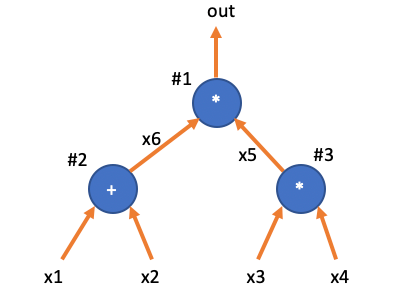
\includegraphics{img/img20230414202348.png}

下面是 \(Q\) 表格

$$
\begin{array}{c|c|c|c|cc}
i & q_L & q_R & q_M & q_C & q_O \\
\hline 0 & 0 & 0 & 0 & 99 & 1 \\
1 & 0 & 0 & 1 & 0 & 1 \\
2 & 1 & 1 & 0 & 0 & 1 \\
3 & 0 & 0 & 1 & 0 & 1
\end{array}
$$

下面是 \(S\) 表格,描述了哪些位置做了置换

\[
\begin{array}{c|c|c|c|}
i & \sigma_{a,i} & \sigma_{b,i} & \sigma_{c,i}  \\
\hline
0 & 0 & 4 & [9] \\
1 & \boxed{10} & \underline{11} & [8] \\
2 & 2 & 6 & \boxed{1} \\
3 & 3 & 7 & \underline{5} \\
\end{array}
\]

\hypertarget{ux5904ux7406-public-inputs}{%
\section{处理 Public Inputs}\label{ux5904ux7406-public-inputs}}

假如在上面给出的小电路中,要证明存在一个 Assignment,使得 out
的输入为一个特定的公开值,比如 \(out=99\)。最简单的办法是使用 \(Q\)
表中的 \(q_C\) 列,并增加一行约束,使得
\(q_L=q_R=q_M=0\),因此满足下面等式

\[
q_C(X) - q_O(X)w_c(X)  = 0
\]

但这个方案的问题是:这些公开值输入输出值被固定成了常数,如果公开值变化,那么
\(q_C(X)\) 多项式需要重新计算。如果整体上 \(W\)
表格的行数比较大,那么这个重新计算过程会带来很多的性能损失。

能否在表格中引入参数,以区分电路中的常数列?并且要求参数的变化并不影响其它电路的部分?这就需要再引入一个新的列,专门存放公开参数,记为
\(\phi\),因此,算术约束会变为:

\[
q_L(X)w_a(X)+q_R(X)w_b(X)+ q_M(X)w_a(X)w_b(X) - q_O(X)w_c(X)+q_C(X)+\phi(X) = 0
\]

我们还可以通过修改拷贝约束的方式引入公开参数。

\begin{quote}
{[}!TODO{]}
\end{quote}

\hypertarget{ux4f4dux7f6eux5411ux91cfux7684ux4f18ux5316}{%
\section{位置向量的优化}\label{ux4f4dux7f6eux5411ux91cfux7684ux4f18ux5316}}

我们上面在构造三个 \(\sigma\) 向量时,直接采用的自然数
\((0,1,2,\cdots)\),这样在协议开始前,Verifier 需要构造 3 个多项式
\(S_{id_a}(X),S_{id_b}(X),S_{id_c}(X)\),并且在协议最后一步查询
Oracle,获得三个多项式在挑战点 \(X=\zeta\) 处的取值
\((S_{id_a}(\zeta),S_{id_b}(\zeta),S_{id_c}(\zeta))\) 。

思考一下, \(\sigma\)
向量只需要用一些互不相等的值来标记置换即可,不一定要采用递增的自然数。如果我们采用
\(H=(1,\omega,\omega^2,\cdots)\) 的话,那么多项式 \({id_a}(X)\)
会被大大简化:

\[
\begin{split}
\vec{id}_a &= (1,\omega,\omega^2,\omega^3)\\
\vec{id}_b &= (k_1,k_1\omega,k_1\omega^2,k_1\omega^3)\\
\vec{id}_c &= (k_2,k_2\omega,k_2\omega^2,k_2\omega^3)\\
\end{split}
\]

其中 \(k_i\) 为互相不等的二次非剩余。

\[
{id_a}(X) = X, \quad {id_b}(X) = k_1\cdot X, \quad  {id_a}(X) = k_2\cdot X
\]

这样一来,这三个多项式被大大简化,它们在 \(X=\zeta\)
处的计算轻而易举,可以直接由 Verifier 完成。

这个小优化手段最早由 Vitalik 提出。采用 \(k_1\) 和 \(k_2\) 是为了产生
\((1,\omega,\omega^2,\omega^3)\) 的陪集(Coset),并保证 Coset
之间没有任何交集。我们前面提到 \(H=(1,\omega,\omega^2,\omega^3)\) 是
\(\mathbb{F}\) 的乘法子群,如果 \(H_1=k_1H\) 和 \(H_2=k_2H\)
存在交集,那么
\(H_1=H_2\)。这个论断可以简单证明如下:如果它们存在交集,那么
\(k_1\omega^i=k_2\omega^j\),于是 \(k_1=k_2\cdot\omega^{j-i}\),又因为
\(\omega^{j-i}\in H\),那么 \(k_1\in H_2\),那么
\(\forall i\in[N]. k_1\cdot \omega^i\in H_2\),那么
\(H_1\subset H_2\),同理可得 \(H_2\subset H_1\),于是 \(H_1=H_2\)。

如果 \(\sigma\) 的列数更多,那么我们需要选择多个 \(k_1, k_2,k_3,\ldots\)
且 \((k_i/k_j)^N\neq1\) 来产生不相交的 Coset。一种最直接的办法是采用
\(k_1,k_2,k_3,\ldots=g^1,g^2,g^3,\ldots\),其中 \(g\) 为乘法子群 \(T\)
的生成元, \(|T|*2^\lambda=p-1\)。

\hypertarget{ux534fux8baeux6846ux67b6}{%
\section{协议框架}\label{ux534fux8baeux6846ux67b6}}

预处理:Prover 和 Verifier 构造 \([q_L(X)]\), \([q_R(X)]\),
\([q_O(X)]\), \([q_M(X)]\), \([q_C(X)]\), \([{\sigma_a}(X)]\),
\([{\sigma_b}(X)]\), \([{\sigma_c}(X)]\)

第一步:Prover 针对 \(W\) 表格的每一列,构造 \([w_a(X)]\),
\([w_b(X)]\), \([w_c(X)]\), \(\phi(X)\) 使得

\[
q_L(X)w_a(X)+q_R(X)w_b(X)+ q_M(X)w_a(X)w_b(X) - q_O(X)w_c(X)+q_C(X) + \phi(X) = 0
\]

第二步: Verifier 发送随机数 \(\beta\) 与 \(\gamma\);

第三步:Prover 构造 \([z(X)]\),使得

\[
\begin{split}
L_0(X)(z(X)-1) &= 0 \\
z(\omega\cdot X)g(X) -  z(X)f(X) &=0
\end{split}
\]

第四步:Verifier 发送随机挑战数 \(\alpha\);

第五步:Prover 计算 \(h(X)\),并构造商多项式 \([t(X)]\)

\[
\begin{split}
h(X) = &\ q_L(X)w_a(X)+q_R(X)w_b(X)+ q_M(X)w_a(X)w_b(X) - q_O(X)w_c(X)+q_C(X) + \phi(X) \\
 & + \alpha(z(\omega X)\cdot g(X)-z(X)\cdot f(X)) + \alpha^2(L_0(X)\cdot(z(X)-1))
\end{split}
\]

其中

\[
\begin{split}
f(X)&=\Big(w_a(X)+\beta\cdot {id_a}(X)+\gamma\Big)\Big(w_b(X)+\beta\cdot {id_b}(X)+\gamma\Big)\Big(w_c(X)+\beta\cdot {id_c}(X)+\gamma\Big)\\
g(X)&=\Big(w_a(X)+\beta\cdot {\sigma_a}(X)+\gamma\Big)\Big(w_b(X)+\beta\cdot {\sigma_b}(X)+\gamma\Big)\Big(w_c(X)+\beta\cdot {\sigma_c}(X)+\gamma\Big)\\
\end{split}
\]

其中商多项式 \(t(X)=\frac{h(X)}{z_H(X)}\) ;

第六步:Verifier 发送随机挑战数 \(\zeta\),查询上述的所有 Oracle,得到 -
\(\bar{w}_a=w_a(\zeta)\), \(\bar{w}_b=w_b(\zeta)\),
\(\bar{w}_c=w_c(\zeta)\) - \(\bar{q}_L=q_L(\zeta)\),
\(\bar{q}_R=q_R(\zeta)\), \(\bar{q}_M=q_M(\zeta)\),
\(\bar{q}_O=q_O(\zeta)\), \(\bar{q}_C=q_C(\zeta)\) -
\(\bar{\sigma}_a=\sigma_a(\zeta)\),
\(\bar{\sigma}_b=\sigma_b(\zeta)\), \(\bar{\sigma}_c=\sigma_c(\zeta)\)
- \(\bar{z}\_{(\omega\cdot\zeta)}=z(\omega\cdot\zeta)\),
\(\bar{z}_{(\zeta)}=z(\zeta)\) - \(\bar{t}=t(\zeta)\)

Verifier 还要自行计算 -
\(\bar{f}_{(\zeta)} =(\bar{w}_a+\beta\cdot \zeta + \gamma) (\bar{w}_b+\beta\cdot k_1\cdot \zeta +\gamma)(\bar{w}_c+\beta\cdot k_2 \cdot \zeta +\gamma)\)
-
\(\bar{g}_{(\zeta)}=(\bar{w}_a+\beta\cdot \bar{\sigma}_1 + \gamma) (\bar{w}_b+\beta\cdot\bar{\sigma}_2+\gamma)(\bar{w}_c+\beta\cdot\bar{\sigma}_3+\gamma)\)
- \(L_0(\zeta)\) - \(z_H(\zeta)\) - \(\phi(\zeta)\)

验证步:

\[
\begin{split}
& \bar{q}_L\bar{w}_a+\bar{q}_R\bar{w}_b+ \bar{q}_M\bar{w}_a\bar{w}_b - \bar{q}_O\bar{w}_c+\bar{q}_C + \phi(\zeta)  \\
& \qquad \qquad + \alpha(\bar{z}\_{(\omega\cdot\zeta)}\cdot \bar{g}\_{(\zeta)}-\bar{z}\_{(\zeta)}\cdot \bar{f}\_{(\zeta)})+ \alpha^2(L_0(\zeta)\cdot(\bar{z}\_{(\zeta)}-1))\overset{?}{=}\bar{t}\cdot z_H(\zeta)
\end{split}
\]

